\documentclass[11pt]{report}
\usepackage{amssymb,amsmath,mathtools,amsthm}
\usepackage[margin=1in]{geometry}
\usepackage{xr-hyper}
\usepackage{hyperref}
\usepackage{graphicx}
\externaldocument{paperlabels}
\newtheorem*{bpstatement}{Statement}
\newcommand{\F}{\mathbb{F}}
\newcommand{\Z}{\mathbb{Z}}
\newcommand{\Tr}{\operatorname{Tr}}
\newcommand{\GR}{\operatorname{GR}}
\newcommand{\red}{\operatorname{red}}
\newcommand{\pending}[1]{\textbf{[#1]}}
\newcommand{\bpmeta}[2]{\par\noindent{\small\textbf{#1:} #2}\par}
\newenvironment{bpcontext}{\par\smallskip\noindent{\small\textit{Paper text (context, verbatim):}}\begin{quote}\small}{\end{quote}}
\sloppy
\title{Blueprint: Explicit reduced APN permutations --- ramification and optimal Galois-ring lifts}
\author{H.~Fukui (generated from the paper source)}
\date{}
\begin{document}
\maketitle
\noindent\textbf{How to read.} Every numbered statement of the paper that carries a label is a node, with its statement and proof copied verbatim from the paper, preceded by the paper's own text around it (setting, notation, admissibility, the definitions of $V,W,Y,Z,D,E$, of $s,\ell,g$, of $R$, coefficient lifts and $\delta_F$, and the normalisation before Proposition~\ref{prop:W}), so that each statement can be read without the paper at hand. Numbers such as ``Theorem~3.1'' are the paper's numbers; citations point to the bibliography at the end, copied from the paper.

\noindent\textbf{Trust labels.} [F] Lean~4 statement checked by the kernel (axioms a subset of propext, Classical.choice, Quot.sound; no sorry), project \texttt{ResidueAPN}. [F (\dots) + M] only the named part is formal; the label note says what is proved in the paper only. [M] proved in the paper only. [L + M] cited result with a self-contained proof in the paper. [Def], [Rem] definitions and remarks.

\noindent\textbf{What the gate checks.} The blueprint gate (\texttt{check\_blueprint.py}) checks that this text, the node list, both graphs and the label file are exactly what the generator produces from the current paper and statement map, that every listed Lean name exists in the sources (a name check, \emph{not} a type check: the types are checked by Lean through the audit files of the release check), and that this PDF was built from those files. It does not check that a prose proof is correct.
\tableofcontents
% content.tex -- GENERATED by gen_blueprint.py; do not edit by hand.
% Statements, proofs and context paragraphs are copied verbatim from the paper source (labels removed).
\setcounter{chapter}{1}\chapter{Preliminaries}
\begin{bpcontext}Throughout, $m\ge5$ is odd, $q=2^m$, and $\sigma(x)=x^2$. For $f\in\F_q[X]$, $\red(f)$ is its reduction modulo $X^q-X$, and $[X^e]f$ denotes the coefficient of $X^e$ in $f$.

A map $f:\F_q\to\F_q$ is \emph{APN} if for every $a\neq0$ and every $b$ the equation $f(x+a)+f(x)=b$ has at most two solutions. A \emph{linearised polynomial} over $\F_q$ is $M=\sum_{i<m}\mu_iX^{2^i}$ with $\mu_i\in\F_q$; the associated map is additive, that is $\F_2$-linear, and every $\F_2$-linear map of $\F_q$ arises in this way. (Only the maps $x\mapsto ax$ are $\F_q$-linear.) The $\F_2$-linear maps commuting with $\sigma$ are the polynomials $\kappa(\sigma)=\sum\kappa_i\sigma^i$ with $\kappa\in\F_2[t]/(t^m-1)$, i.e.\ the linearised polynomials with coefficients in $\F_2$; $\kappa(\sigma)$ is bijective iff $\gcd(\kappa,t^m-1)=1$.

A \emph{Dembowski--Ostrom (DO) polynomial} is an $\F_q$-linear combination of monomials $X^{2^i+2^j}$, $0\le i<j<m$. A \emph{quadratic} polynomial is a DO polynomial plus a linearised polynomial plus a constant. The derivative of $X^{2^i+2^j}$ is $X^{2^j}$ if $i=0$ and $0$ otherwise, and that of $X^{2^i}$ is $1$ if $i=0$ and $0$ otherwise. Hence for quadratic $p$,
\begin{equation}\tag{\ref*{eq:der}}
p'=\epsilon+K(X),\qquad \epsilon=[X]p\in\F_q,\quad K=\sum_{j\ge1}([X^{1+2^j}]p)\,X^{2^j}\ \text{linearised}.
\end{equation}\end{bpcontext}
\section*{Definition~\ref{def:opt}}\label{bp:def:opt}
\addcontentsline{toc}{section}{Definition \ref{def:opt} \quad[Def]}
\bpmeta{Trust}{[Def]}
\bpmeta{Lean definitions}{\texttt{ResidueAPN.\allowbreak{}IsDerivOptimal}, \texttt{ResidueAPN.\allowbreak{}IsOptimalAPNPerm}, \texttt{ResidueAPN.\allowbreak{}IsAPN}}
\bpmeta{Label note}{definition; the Lean definitions are read against the paper in MEANING\_MAP.md (every nonempty fibre has two elements = the fibre through each point has two elements).}
\begin{bpstatement}
A reduced $p\in\F_q[X]$ is \emph{derivative-optimal} if $p'$ has no zero on $\F_q$ and every nonempty fibre of $x\mapsto p'(x)$ on $\F_q$ has two elements. An \emph{optimal APN permutation} is an APN permutation of $\F_q$ whose reduced polynomial is derivative-optimal.
\end{bpstatement}
\begin{bpcontext}For quadratic $p$, \eqref{eq:der} shows that $p$ is derivative-optimal iff $\ker K=\{0,\rho\}$ for some $\rho\ne0$ and $\epsilon\notin K(\F_q)$; the fibres of $p'$ are the cosets $\{x,x+\rho\}$.\end{bpcontext}
\section*{Lemma~\ref{lem:O}}\label{bp:lem:O}
\addcontentsline{toc}{section}{Lemma \ref{lem:O} \quad[F]}
\bpmeta{Trust}{[F]}
\bpmeta{Lean theorems}{\texttt{ResidueAPN.\allowbreak{}lemma\_\allowbreak{}2\_\allowbreak{}2}, \texttt{ResidueAPN.\allowbreak{}lemma\_\allowbreak{}2\_\allowbreak{}2\_\allowbreak{}core}, \texttt{ResidueAPN.\allowbreak{}derivative\_\allowbreak{}quadratic}, \texttt{ResidueAPN.\allowbreak{}card\_\allowbreak{}kerL\_\allowbreak{}of\_\allowbreak{}dvd}}
\bpmeta{Label note}{formal (stage 3, session R11) for every polynomial over F\_2 with quadratic support (IsQuadSupp: exponents 0, 2\textasciicircum{}i, 2\textasciicircum{}i+2\textasciicircum{}j, i<j<m) over F = F\_\{2\textasciicircum{}m\}, m odd; display (1) for F\_2 coefficients is derivative\_quadratic; gcd is EuclideanDomain.gcd in F\_2[t] (its only unit is 1, so this is the monic gcd). The formal proof does not use a normal basis: \#ker phi(sigma) = 2\textasciicircum{}(deg phi) for phi dividing t\textasciicircum{}m-1, from a root bound and \#ker (phi psi)(sigma) $\le$ \#ker phi(sigma) \#ker psi(sigma); ker kappa(sigma) = ker g(sigma) by Bezout. The hypothesis 'reduced' is not needed.}
\begin{bpstatement}
Let $p$ be a reduced quadratic polynomial with coefficients in $\F_2$, and let $\kappa\in\F_2[t]$ be the polynomial $\sum_{j\ge1}([X^{1+2^j}]p)\,t^j$, so that $K=\kappa(\sigma)$. Then $p$ is derivative-optimal iff $\epsilon=1$ and $\gcd(\kappa,t^m-1)=t+1$.
\end{bpstatement}
\begin{proof}
Fix a normal element $\beta$; then $f\mapsto f(\sigma)\beta$ identifies $\F_2[t]/(t^m-1)$ with $\F_q$, and $\kappa(\sigma)$ becomes multiplication by $\kappa$. Its kernel has dimension $\deg\gcd(\kappa,t^m-1)$ and its image is the ideal generated by this gcd. The fibres of $p'$ have size two iff the gcd has degree one, i.e.\ equals $t+1$. If $\epsilon=0$, $0$ is a value. If $\epsilon=1$: $\Tr(\beta)=1$ (the conjugates of a normal element are linearly independent, so their sum is not $0$), so $1=\sum_i\sigma^i\beta$ corresponds to $1+t+\dots+t^{m-1}$, which is not in $(t+1)$ since its value at $1$ is $m\equiv1$.
\end{proof}
\setcounter{chapter}{2}\chapter{The family}
\noindent Paper: Section~\ref{sec:A}.
\begin{bpcontext}Call an odd $r$ with $3\le r<m$ and $\gcd(r,m)=1$ \emph{admissible} ($r=m-2$ always is). Put $T_r=\sum_{i<r}X^{2^i}$ and
\begin{gather*}
V=\sum_{i=0}^{r-3}X^{2^i},\quad W=X^{2^{r-2}},\quad Y=X^{2^{m-2}},\quad Z=X^{2^{m-1}},\\
D=1+W+Y,\quad E=1+V+Y+Z.
\end{gather*}\end{bpcontext}
\section*{Theorem~\ref{thm:A}}\label{bp:thm:A}
\addcontentsline{toc}{section}{Theorem \ref{thm:A} \quad[F]}
\bpmeta{Trust}{[F]}
\bpmeta{Cites (earlier labelled statements)}{\hyperref[bp:lem:O]{Lemma~\ref*{lem:O}}}
\bpmeta{Lean theorems}{\texttt{ResidueAPN.\allowbreak{}theorem\_\allowbreak{}3\_\allowbreak{}1}, \texttt{ResidueAPN.\allowbreak{}polP\_\allowbreak{}eq\_\allowbreak{}sum\_\allowbreak{}supp}, \texttt{ResidueAPN.\allowbreak{}card\_\allowbreak{}suppP}, \texttt{ResidueAPN.\allowbreak{}natDegree\_\allowbreak{}polP}, \texttt{ResidueAPN.\allowbreak{}eval\_\allowbreak{}polP}, \texttt{ResidueAPN.\allowbreak{}isOptimalAPNPerm\_\allowbreak{}P}, \texttt{ResidueAPN.\allowbreak{}image\_\allowbreak{}evalD}}
\bpmeta{Label note}{all four items; Tr is written as the sum of Frobenius powers (absTr).}
\begin{bpstatement}
Let $r$ be admissible and $P_{m,r}:=\red\bigl((T_r^3)^{2^{m-2}}\bigr)$; we write $P=P_{m,r}$ when $(m,r)$ is fixed.
\begin{enumerate}
\item $P_{m,r}=V+W+WV+WY+WZ+YV+YZ$; it has coefficients in $\F_2$, exactly $3r-2$ terms and degree $3q/4$.
\item As a map of $\F_q$, $P_{m,r}=\sigma^{m-2}\circ X^3\circ T_r$; it is an APN permutation.
\item $P'_{m,r}=D=1+X^{2^{r-2}}+X^{2^{m-2}}$; $P_{m,r}$ is derivative-optimal, with fibres $\{x,x+1\}$ and image of $P'_{m,r}$ equal to $1+\ker\Tr$.
\item $P_{m,r}+1=D\cdot E$ in $\F_2[X]$, and $E'=1$.
\end{enumerate}
\end{bpstatement}
\begin{proof}
(2) $T_r$ is $\tau(\sigma)$ with $\tau=(t^r-1)/(t-1)$. Since $\gcd(t^r-1,t^m-1)=t-1$ and $\tau(1)=r\equiv1$, $\tau$ is a unit and $T_r$ is bijective. $X^3$ is an APN permutation of $\F_q$ for odd $m$, and $\sigma^{m-2}$ is additive and bijective; composing with additive bijections on both sides preserves both properties.

(1) $T_r^3=T_r^2T_r=\sum_{i,j<r}X^{2^{i+1}+2^j}$. The diagonal pairs $i+1=j$ give the linear terms $X^{2\cdot2^j}=X^{2^{j+1}}$ ($1\le j\le r-1$). A two-element set $\{a,b\}\subseteq[1,r-1]$ arises from $(i+1,j)=(a,b)$ and from $(b,a)$ and cancels; the survivors are $\{0,b\}$ ($1\le b\le r$) and $\{a,r\}$ ($1\le a\le r-1$); the set $\{0,r\}$ occurs once, from $(i+1,j)=(r,0)$. So $T_r^3$ has $r-1$ linear and $2r-1$ quadratic terms, all of degree $<q$. Raising to the power $2^{m-2}$ and reducing rotates every index by $-2$ modulo $m$, injectively. The result has the linear terms $X^{2^i}$, $0\le i\le r-2$ ($=V+W$), and the quadratic terms with index sets $\{m-2,b-2\}$, $1\le b\le r$, and $\{a-2,r-2\}$, $1\le a\le r-1$, which are the supports of $YZ$, $YV$, $WY$ and of $WZ$, $WV$. The count is $3r-2$; the largest exponent is $2^{m-1}+2^{m-2}=3q/4$.

(3) The odd exponents are $1$ (in $V$), $2^{r-2}+1$ (in $WV$) and $2^{m-2}+1$ (in $YV$), so $P'=D$. Here $\kappa=t^{r-2}+t^{m-2}=t^{r-2}(1+t^{m-r})$ and $\gcd(\kappa,t^m-1)=t^{\gcd(m-r,m)}-1=t+1$; Lemma~\ref{lem:O} applies. Directly, $x^{2^{r-2}}+x^{2^{m-2}}=(x^{2^r}+x)^{2^{m-2}}$ has kernel $\F_2$ and image $\ker\Tr$.

(4) In $\F_2[X]$, $DE=1+V+W+Z+WV+WY+WZ+YV+Y^2+YZ$ (the two terms $Y$ cancel), and $Y^2=Z$; hence $DE=1+P_{m,r}$. $E'=V'=1$.
\end{proof}
\begin{bpcontext}\subsection*{Why the inner map is not a monomial}\end{bpcontext}
\section*{Lemma~\ref{lem:LW} (Li--Wang {\cite[Thm.~4]{LW}})}\label{bp:lem:LW}
\addcontentsline{toc}{section}{Lemma \ref{lem:LW} \quad[L + M]}
\bpmeta{Trust}{[L + M]}
\bpmeta{Label note}{cited (Li-Wang, DCC 2011, Thm. 4); self-contained proof in the paper; not formalized. Not required: Section 3 comparison, not a dependency of the formal statements of A, B, C, R, W (GPT R7).}
\begin{bpstatement}
Let $1\le h<m$ with $\gcd(h,m)=1$ and let $M=\sum_{i<m}\mu_iX^{2^i}$ be a reduced linearised polynomial over $\F_q$. Then $X^{2^h+1}+M$ permutes $\F_q$ iff $M=\gamma^{2^h}X+\gamma X^{2^h}$ for some $\gamma\in\F_q$, i.e.\ $X^{2^h+1}+M=(X+\gamma)^{2^h+1}+\gamma^{2^h+1}$.
\end{bpstatement}
\begin{bpcontext}Li and Wang state this for nonzero $M$, i.e.\ $\gamma\neq0$; $\gamma=0$ is the Gold function itself, a permutation since $m$ is odd. They write out the proof for $h=1$ \cite[Thm.~2]{LW}, where the binary weights of the relevant exponents already separate the cyclotomic classes, and note that it extends to $\gcd(h,m)=1$. For general $h$ two classes can have the same weight, so we give a short self-contained proof that includes this comparison.\end{bpcontext}
\begin{proof}
For $a\ne0$ and $z=x/a$, $(x+a)^{2^h+1}+x^{2^h+1}+M(a)=a^{2^h+1}(z^{2^h}+z+1)+M(a)$, and $z^{2^h}+z$ ranges over $\ker\Tr$ (its kernel is $\F_{2^{\gcd(h,m)}}=\F_2$; this is the only use of $\gcd(h,m)=1$). As $\Tr(1)=1$ ($m$ odd), $X^{2^h+1}+M$ is a permutation iff $\Tr\bigl(M(a)a^{-(2^h+1)}\bigr)=0$ for all $a\ne0$. With $c_i=2^i-2^h-1$ this reads $\sum_i\Tr(\mu_ia^{c_i})=0$ on $\F_q^*$. Modulo $Q=q-1$, multiplication by $2$ rotates $m$-bit words (bit $j$ is the coefficient of $2^j$); the orbits of $c\mapsto2c$ on $\Z/Q$ are the cyclotomic classes. The word of $c_h=-1$ has its only zero at position $0$, that of $c_0=-2^h$ at position $h$, so $c_0=2^hc_h$. For $0<i<h$ the ones of $c_i$ occupy $[1,i-1]\cup[h,m-1]$ (weight $m-h+i-1$), for $h<i<m$ they occupy $[0,h-1]\cup[h+1,i-1]$ (weight $i-1$); both weights are at most $m-2$. Every such word contains both digits and has one or two cyclic runs of zeros. A word fixed by a nontrivial rotation consists of $m/d$ copies of a block, $d$ a proper divisor of the odd number $m$, so its number of zero runs would be a positive multiple of $m/d\ge3$; hence every class has $m$ elements, and none is the class of $0$. Words of different weight lie in different classes, so it remains to compare $c_u$ and $c_v$ with $0<u<h<v=m-h+u$. Their zero sets are $\{0\}\cup[u,h-1]$ and $\{h\}\cup[v,m-1]$; the first is a single run iff $u=1$, the second iff $v=h+1$, and both happen only if $m=2h$. If exactly one of them is a single run, the two words have different numbers of zero runs and lie in different classes. Otherwise ($u\ge2$, $v\ge h+2$) both have zero runs of lengths $1$ and $h-u$. If $h-u\ge2$, a rotation matches the isolated zeros, and the runs of ones that follow them have lengths $u-1$ and $v-h-1$, so $v=u+h$ and $m=2h$. If $h-u=1$, the gaps between the two zeros are $\{h-2,m-h\}$ and $\{h,m-h-2\}$, equal only if $m=2h$. As $m$ is odd, the classes of the $c_i$, $i\ne0,h$, are pairwise distinct and distinct from that of $c_h$. So the left side is a polynomial in $a$ with exponents in $[1,Q-1]$ whose coefficients are $\mu_i^{2^j}$ at $a^{c_i2^j}$, except on the class of $c_h$, where they are $\mu_h^{2^j}+\mu_0^{2^{j-h}}$. A polynomial of degree $<Q$ vanishing on $\F_q^*$ is zero; hence $\mu_i=0$ for $i\notin\{0,h\}$ and $\mu_0=\mu_h^{2^h}$, i.e.\ $M=\gamma^{2^h}X+\gamma X^{2^h}$ with $\gamma=\mu_h$. Conversely, for such $M$ the identity in the statement and the bijectivity of $X^{2^h+1}$ ($m$ odd) show that $X^{2^h+1}+M$ permutes $\F_q$.
\end{proof}
\section*{Corollary~\ref{cor:P}}\label{bp:cor:P}
\addcontentsline{toc}{section}{Corollary \ref{cor:P} \quad[M]}
\bpmeta{Trust}{[M]}
\bpmeta{Cites (earlier labelled statements)}{\hyperref[bp:lem:LW]{Lemma~\ref*{lem:LW}}}
\bpmeta{Label note}{not formalized; not required (see Lemma 3.2).}
\begin{bpstatement}
Let $G=X^{2^h+1}$ with $\gcd(h,m)=1$, let $N$ be an $\F_2$-linear bijection and $L$ an $\F_2$-linear map of $\F_q$, $b\in\F_q^*$ and $0\le j<m$. No permutation of the form $N\circ G\circ(bX^{2^j})+L+\text{const}$ is derivative-optimal. Hence an optimal APN permutation in the extended-affine class of $G$, written $N\circ G\circ B+L+\text{const}$ with $B$ an $\F_2$-linear bijection (an inner translation only adds an affine map, as $G$ is quadratic), has an inner map $B$ that is not a monomial.
\end{bpstatement}
\begin{proof}
$G\circ(bX^{2^j})=b^{2^h+1}\sigma^j\circ G$, and $N\circ(b^{2^h+1}\sigma^j)$ is again an $\F_2$-linear bijection, so it suffices to treat $N\circ G+L$. If it permutes $\F_q$, so does $G+N^{-1}L$, and Lemma~\ref{lem:LW} gives $N\circ G+L=H(X+\gamma)+\text{const}$ with $H=\red(N\circ G)$. As $\deg H<q$, $H(X+\gamma)$ is reduced, and its formal derivative is $H'(X+\gamma)$. Every exponent of $H$ has binary weight two, so $H$ has no term $X$ and $H'(0)=0$ by \eqref{eq:der}; the derivative $H'(X+\gamma)$ of the permutation vanishes at $\gamma$.
\end{proof}
\begin{bpcontext}For $m\ge5$ and representations without affine part the inner map is determined up to a monomial: replacing $h$ by $m-h$ changes $G$ only by a power of $\sigma$ on the output, so we may assume $h<m/2$, and if $N_1\circ G\circ B_1=N_2\circ G\circ B_2$, then $B_1B_2^{-1}$ is a monomial $aX^{2^u}$ \cite[Thm.~4.1]{KZ}. With affine parts the corresponding statement concerns the extended-affine automorphism group of $G$; we do not use it. In Theorem~\ref{thm:A} the inner map is $T_r$.\end{bpcontext}
\setcounter{chapter}{3}\chapter{Ramification}
\noindent Paper: Section~\ref{sec:B}.
\begin{bpcontext}Let $s=m-r$ (even), $\ell=2^{r-2}$ and $g=X^{2^s}+X+1\in\F_2[X]$. We regard $P=P_{m,r}$ as a map $\mathbb P^1\to\mathbb P^1$ over $\overline{\F}_2$ of degree $n=3q/4$; it is separable, as $P'\ne0$. At a finite point $\alpha$, the ramification index $e_\alpha$ is the multiplicity of $\alpha$ as a root of $P-P(\alpha)$, and the different exponent is $d_\alpha=\operatorname{ord}_\alpha P'$; in characteristic two $d_\alpha\ge e_\alpha$ when $e_\alpha$ is even (wild ramification), so $d_\alpha$ is not $e_\alpha-1$ in general. A \emph{ramification point} is a point with $e_\alpha>1$; its image is a \emph{branch value}.\end{bpcontext}
\section*{Theorem~\ref{thm:B}}\label{bp:thm:B}
\addcontentsline{toc}{section}{Theorem \ref{thm:B} \quad[F (items (1)-(3), root multiplicities) + M]}
\bpmeta{Trust}{[F (items (1)-(3), root multiplicities) + M]}
\bpmeta{Cites (earlier labelled statements)}{\hyperref[bp:thm:A]{Theorem~\ref*{thm:A}}}
\bpmeta{Lean theorems}{\texttt{ResidueAPN.\allowbreak{}derivative\_\allowbreak{}polP\_\allowbreak{}eq\_\allowbreak{}pow}, \texttt{ResidueAPN.\allowbreak{}polP\_\allowbreak{}add\_\allowbreak{}one\_\allowbreak{}eq\_\allowbreak{}pow}, \texttt{ResidueAPN.\allowbreak{}separable\_\allowbreak{}polG}, \texttt{ResidueAPN.\allowbreak{}root\_\allowbreak{}fixed\_\allowbreak{}two\_\allowbreak{}s}, \texttt{ResidueAPN.\allowbreak{}root\_\allowbreak{}not\_\allowbreak{}fixed\_\allowbreak{}s}, \texttt{ResidueAPN.\allowbreak{}root\_\allowbreak{}not\_\allowbreak{}fixed\_\allowbreak{}of\_\allowbreak{}coprime}, \texttt{ResidueAPN.\allowbreak{}card\_\allowbreak{}roots\_\allowbreak{}polG}, \texttt{ResidueAPN.\allowbreak{}isCoprime\_\allowbreak{}polG\_\allowbreak{}polE}, \texttt{ResidueAPN.\allowbreak{}multiplicity\_\allowbreak{}at\_\allowbreak{}root}, \texttt{ResidueAPN.\allowbreak{}derivative\_\allowbreak{}eval\_\allowbreak{}eq\_\allowbreak{}zero\_\allowbreak{}iff}}
\bpmeta{Label note}{formal: P' = g\textasciicircum{}l, P+1 = g\textasciicircum{}l E, g separable with 2\textasciicircum{}s roots in F\_\{2\textasciicircum{}\{2s\}\} minus (F\_\{2\textasciicircum{}s\} union F\_q), gcd(g,E)=1 over F\_2, P = 1 at the roots, multiplicity l as a root of P+1 and of P'. Paper only: reading these multiplicities as ramification indices / different exponents of P\textasciicircum{}1 $\to$ P\textasciicircum{}1, the point at infinity (Riemann-Hurwitz), the fibre over 1.}
\begin{bpstatement}
\begin{enumerate}
\item $P_{m,r}'=g^{\ell}$ and $P_{m,r}+1=g^{\ell}E$.
\item $g$ is separable; its $2^s$ roots lie in $\F_{2^{2s}}\setminus(\F_{2^s}\cup\F_q)$.
\item $\gcd(g,E)=1$.
\end{enumerate}
Consequently the finite ramification points are the $2^s$ roots of $g$; each has $e_\alpha=\ell$ and $d_\alpha=\ell$ and maps to $1$. The point $\infty$ has $e_\infty=n$ and $d_\infty=2n-2-\deg P'=5q/4-2$. The branch values are exactly $1$ and $\infty$. The fibre over $1$ consists of the roots of $g$ and $2^{m-1}$ simple points, exactly one of which is $\F_q$-rational.
\end{bpstatement}
\begin{proof}
(1) $g^{\ell}=X^{2^{m-2}}+X^{2^{r-2}}+1=D$; use Theorem~\ref{thm:A}(3),(4). (2) $g'=1$. If $g(\alpha)=0$ then $\alpha^{2^s}=\alpha+1$, so $\alpha\notin\F_{2^s}$ and $\alpha^{2^{2s}}=\alpha$. As $\gcd(2s,m)=1$, $\F_{2^{2s}}\cap\F_q=\F_2$, and $g(0)=g(1)=1$. (3) Modulo $g$, $X^{2^{s+j}}\equiv X^{2^j}+1$, so $Y\equiv X^{2^{r-2}}+1$, $Z\equiv X^{2^{r-1}}+1$ and $E\equiv1+T_r$. If $g(\alpha)=T_r(\alpha)+1=0$, then $T_r^2+T_r=X+X^{2^r}$ gives $\alpha^{2^r}=\alpha$, so $\alpha\in\F_{2^{\gcd(r,2s)}}=\F_2$ ($r$ odd, $\gcd(r,s)=\gcd(r,m)=1$), contradicting $g(0)=g(1)=1$.

$P'$ vanishes only at the roots of $g$, so these are the only finite ramification points. At a root $\alpha$, $P(\alpha)=1$ by (1), and $\alpha$ is a root of multiplicity exactly $\ell$ of $P+1=g^{\ell}E$, since $g$ is separable and $E(\alpha)\neq0$ by (3); so $e_\alpha=\ell$, and $d_\alpha=\operatorname{ord}_\alpha g^{\ell}=\ell$. Riemann--Hurwitz for the separable degree-$n$ map of genus zero gives $\sum_\alpha d_\alpha+d_\infty=2n-2$; the finite sum is $2^s\ell=q/4=\deg P'$, so $d_\infty=3q/2-2-q/4=5q/4-2$, and $e_\infty=n$ since $P$ is a polynomial. $E$ has degree $2^{m-1}$, is separable ($E'=1$), and $P'=g^\ell$ does not vanish at its roots by (3), so they are simple points of the fibre over $1$; the degrees match, $2^s\ell+2^{m-1}=q/4+q/2=n$. As $P$ permutes $\F_q$, $P(x)=1$ has exactly one rational solution, which is not a root of $g$ by (2).
\end{proof}
\begin{bpcontext}All ramification is wild ($\ell$ and $n$ are even), and at the finite points $d_\alpha=e_\alpha$ is the least value allowed for wild ramification. Galois closures, monodromy and higher ramification groups are not determined here. For $r=m-2$ the finite ramification points are the four roots of $X^4+X+1$ for every $m$.\end{bpcontext}
\section*{Remark~\ref{rem:tit} (comparison with \cite{TIT})}\label{bp:rem:tit}
\addcontentsline{toc}{section}{Remark \ref{rem:tit} \quad[Rem]}
\bpmeta{Trust}{[Rem]}
\bpmeta{Cites (earlier labelled statements)}{\hyperref[bp:thm:A]{Theorem~\ref*{thm:A}}}
\bpmeta{Label note}{remark with a computation; not formalized.}
\begin{bpstatement}
Let $1\le e\le(m-1)/2$, $\theta\in\F_q^\times$ with $\Tr(\theta)=0$, $L_\theta=\sum_i\theta^{2^i}X^{2^i}$ and $P_{e,\theta}=X^{2^{e+1}+2}+(X^{2^{e+1}}+X^2+1)L_\theta$. If $\gcd(e,m)=1$, $P_{e,\theta}$ is, by \cite[App.~A]{TIT}, an optimal APN permutation linearly equivalent to $X^{2^e+1}$. Without this condition it need not be APN or derivative-optimal: for $m=9$, $e=3$ and $\theta$ a root of the irreducible polynomial $X^9+X^4+1$ (its trace is $0$), $P_{e,\theta}$ permutes $\F_q$, but its differential uniformity is $8$ and the nonempty fibres of $P_{e,\theta}'$ have $8$ elements. The count of branch values below uses neither condition. Put $g_e=X^{2^e}+X+1$, so $g_e^2=X^{2^{e+1}}+X^2+1$ and $P_{e,\theta}'=\theta\,g_e^2$. At a root $\alpha$ of $g_e$, $P_{e,\theta}(\alpha)=\alpha^{2^{e+1}+2}=(\alpha^2+\alpha)^2$, using $\alpha^{2^e}=\alpha+1$. The roots form a coset $\alpha_0+\F_{2^e}$, and $u\mapsto(\alpha_0+u)^2+(\alpha_0+u)=(\alpha_0^2+\alpha_0)+(u^2+u)$ is two-to-one onto a coset of the trace-zero hyperplane of $\F_{2^e}$; squaring is injective. Hence the finite branch values of $P_{e,\theta}$ are exactly $2^{e-1}$ in number. For $e=1$ there is one, and explicitly
\[
P_{1,\theta}+1=(X^2+X+1)^2\bigl((X+1)^2+L_\theta\bigr).
\]
So a single finite branch value is not special to Theorem~\ref{thm:A}: the maps $P_{1,\theta}$, which lie in the class of $X^3$ like $P_{m,r}$, have it, with coefficients outside $\F_2$ ($\Tr(\theta)=0$ excludes $\theta=1$) and two finite critical points. Theorem~\ref{thm:A} has coefficients in $\F_2$ and $2^{m-r}$ critical points of index $2^{r-2}$.
\end{bpstatement}
\setcounter{chapter}{4}\chapter{The integer product form}
\noindent Paper: Section~\ref{sec:C}.
\section*{Proposition~\ref{prop:C}}\label{bp:prop:C}
\addcontentsline{toc}{section}{Proposition \ref{prop:C} \quad[F (identity) + M]}
\bpmeta{Trust}{[F (identity) + M]}
\bpmeta{Cites (earlier labelled statements)}{\hyperref[bp:thm:A]{Theorem~\ref*{thm:A}}}
\bpmeta{Lean theorems}{\texttt{ResidueAPN.\allowbreak{}proposition\_\allowbreak{}5\_\allowbreak{}1}, \texttt{ResidueAPN.\allowbreak{}lift\_\allowbreak{}reduces}}
\bpmeta{Label note}{the identity in Z[X] and its image in every commutative ring are formal; the operation count is paper only.}
\begin{bpstatement}
Let $\hat P\in\Z[X]$ be the $0/1$ lift of $P_{m,r}$ and $\hat V,\hat W,\hat Y,\hat Z,\hat D,\hat E$ the $0/1$ lifts of $V,\dots,E$. Then
\[
\hat P=\hat D\hat E-1-2(\hat Y+\hat Z)\quad\text{in }\Z[X].
\]
Over every Galois ring $\GR(2^k,m)$, $k\ge1$, $\hat P(x)$ can be evaluated with $m-1$ squarings, one general multiplication and $r+5$ additions or subtractions.
\end{bpstatement}
\begin{proof}
In $\Z[X]$, $\hat D\hat E=1+\hat V+\hat W+2\hat Y+\hat Z+\hat W\hat V+\hat W\hat Y+\hat W\hat Z+\hat Y\hat V+\hat Y^2+\hat Y\hat Z$ and $\hat Y^2=\hat Z$. Hence $\hat D\hat E-1-2(\hat Y+\hat Z)=\hat V+\hat W+\hat W\hat V+\hat W\hat Y+\hat W\hat Z+\hat Y\hat V+\hat Y\hat Z$; its monomials are pairwise distinct with coefficient $1$, and by Theorem~\ref{thm:A}(1) this is $\hat P$. Schedule: $x^{2^i}$ for $1\le i\le m-1$ by squaring; $S=\hat Y+\hat Z$ (one addition), $\hat D=1+\hat W+\hat Y$ (two), $\hat E=(1+\hat V)+S$ ($r-1$), $\hat D\hat E$ (one multiplication), $\hat D\hat E-(1+S+S)$ (three). Squarings in the ring are counted as operations, not as free.
\end{proof}
\begin{bpcontext}This is an upper bound for the natural lift. We do not claim that it is minimal, and we say nothing about the cost of a complete cipher.\end{bpcontext}
\setcounter{chapter}{5}\chapter{Coefficient lifts}
\noindent Paper: Section~\ref{sec:ring}.
\begin{bpcontext}Let $R=\GR(2^k,m)$, $k\ge2$, with residue map $x\mapsto\bar x$ onto $\F_q$. For $p\in\F_q[X]$, a \emph{coefficient lift} is any $F\in R[X]$ with $\bar F=p$. Differences are taken in $R$: for $\alpha,\beta\in R$, $\delta_F(\alpha,\beta)=\#\{x\in R:F(x+\alpha)-F(x)=\beta\}$, and $\Delta_F=\max_{\alpha\ne0,\beta}\delta_F(\alpha,\beta)$.\end{bpcontext}
\section*{Proposition~\ref{prop:lift}}\label{bp:prop:lift}
\addcontentsline{toc}{section}{Proposition \ref{prop:lift} \quad[F (abstract finite local ring) + M]}
\bpmeta{Trust}{[F (abstract finite local ring) + M]}
\bpmeta{Lean theorems}{\texttt{ResidueAPN.\allowbreak{}prop\_\allowbreak{}6\_\allowbreak{}1}, \texttt{ResidueAPN.\allowbreak{}prop\_\allowbreak{}6\_\allowbreak{}1\_\allowbreak{}family}}
\bpmeta{Label note}{formal for every finite commutative ring R with a surjection pi onto F such that elements outside ker pi are units; that GR(2\textasciicircum{}k,m) is such a ring is paper level (Galois rings are not in Mathlib).}
\begin{bpstatement}
If $p$ permutes $\F_q$ and $p'$ has no zero on $\F_q$, every coefficient lift of $p$ permutes $R$.
\end{bpstatement}
\begin{proof}
If $F(x)=F(y)$, then $p(\bar x)=p(\bar y)$, so $y=x+\eta$ with $\eta\in2R$. If $\eta\neq0$, let $\eta\in2^jR\setminus2^{j+1}R$, $j\ge1$. Then $F(x+\eta)-F(x)=\eta F'(x)+\eta^2H_0$ with $H_0\in R$; $F'(x)$ is a unit since $\overline{F'(x)}=p'(\bar x)\ne0$, so $\eta F'(x)\notin2^{j+1}R$, while $\eta^2H_0\in2^{2j}R\subseteq2^{j+1}R$. Hence $F(x+\eta)\ne F(x)$.
\end{proof}
\begin{bpcontext}This is the sufficiency half of \cite[Thm.~2]{RS}, included for completeness.\end{bpcontext}
\section*{Theorem~\ref{thm:R}}\label{bp:thm:R}
\addcontentsline{toc}{section}{Theorem \ref{thm:R} \quad[F (abstract finite local ring) + M]}
\bpmeta{Trust}{[F (abstract finite local ring) + M]}
\bpmeta{Lean theorems}{\texttt{ResidueAPN.\allowbreak{}thm\_\allowbreak{}6\_\allowbreak{}2\_\allowbreak{}unit}, \texttt{ResidueAPN.\allowbreak{}thm\_\allowbreak{}6\_\allowbreak{}2\_\allowbreak{}unit\_\allowbreak{}family}, \texttt{ResidueAPN.\allowbreak{}thm\_\allowbreak{}6\_\allowbreak{}2\_\allowbreak{}top}, \texttt{ResidueAPN.\allowbreak{}thm\_\allowbreak{}6\_\allowbreak{}2\_\allowbreak{}top\_\allowbreak{}family}, \texttt{ResidueAPN.\allowbreak{}card\_\allowbreak{}ker\_\allowbreak{}mul}, \texttt{ResidueAPN.\allowbreak{}card\_\allowbreak{}fibre}}
\bpmeta{Label note}{(1) for pi(alpha) outside \{0,1\} = ker K; (2) for alpha in ker pi with annihilator ker pi (nonzero top-ideal elements of GR(2\textasciicircum{}k,m), k$\ge$2); the count 2 q\textasciicircum{}(k-1) is 2 \#(ker pi), and \#R = \#F \#(ker pi). card\_fibre: every fibre of pi has \#(ker pi) elements. Paper only (GR\_BRIDGE.md): the Galois-ring instance (B1-B4); the number (q-2)q\textasciicircum{}(k-1) of directions in (1), which is (q-2)\#(ker pi) with \#(ker pi) = q\textasciicircum{}(k-1); the RS-cited bounds after the theorem.}
\begin{bpstatement}
Let $p$ be a quadratic optimal APN permutation of $\F_q$, with $p'=\epsilon+K$ as in \eqref{eq:der} and $\ker K=\{0,\rho\}$, and let $F$ be any coefficient lift.
\begin{enumerate}
\item (Unit directions off $\rho$.) If $\bar\alpha\notin\{0,\rho\}$, then $\delta_F(\alpha,\beta)=\#\{y\in\F_q:p(y+\bar\alpha)+p(y)=\bar\beta\}\le2$ for every $\beta\in R$. There are $(q-2)q^{k-1}$ such $\alpha$.
\item (Top ideal.) If $\alpha\in2^{k-1}R\setminus\{0\}$, then every nonzero entry $\delta_F(\alpha,\beta)$ equals $2q^{k-1}$.
\end{enumerate}
\end{bpstatement}
\begin{proof}
(1) Put $\mathcal D(X)=F(X+\alpha)-F(X)-\beta$. Its reduction is $p(X+\bar\alpha)+p(X)+\bar\beta$, whose derivative $p'(X+\bar\alpha)+p'(X)=K(\bar\alpha)$ is a nonzero constant. So every root of the reduction in $\F_q$ is simple and lifts to exactly one root of $\mathcal D$ in $R$ (Hensel), and every root of $\mathcal D$ reduces to a root. The bound $2$ is the APN property of $p$.
(2) Write $\alpha=2^{k-1}u$, $u$ a unit. By Taylor expansion with integer binomial coefficients, $F(x+\alpha)-F(x)=\alpha F'(x)+\alpha^2(\dots)=\alpha F'(x)$, as $\alpha^2=0$ for $k\ge2$. Since $\alpha\cdot2R=0$, $\alpha F'(x)$ depends only on $\bar x$ and corresponds to $\bar u\,p'(\bar x)$ under $2^{k-1}R\cong\F_q$ (multiplication by $2^{k-1}$ induces an additive isomorphism $R/2R\to2^{k-1}R$, as the annihilator of $2^{k-1}$ in $R$ is $2R$). The map $\bar x\mapsto\bar u\,p'(\bar x)$ is two-to-one onto its image, and each residue class has $q^{k-1}$ elements.
\end{proof}
\begin{bpcontext}Part~(2) of the theorem uses only that $p$ is derivative-optimal; part~(1) uses that $p$ is quadratic and APN with $\ker K=\{0,\rho\}$. The theorem gives exact rows in these two classes of directions. In the remaining directions only upper bounds are used, from \cite{RS}: if $\bar\alpha=\rho$, \cite[Prop.~4(1)]{RS} gives $\delta_F(\alpha,\beta)\le2q^{k-1}$; if $\alpha\in2R\setminus2^{k-1}R$, \cite[Prop.~5]{RS}, applied with the fibres of $p'$ of size two, gives the same bound. Since by part~(2) some entry equals $2q^{k-1}$, $\Delta_F=2q^{k-1}$ for every coefficient lift; this is the ring corollary of \cite{TIT} (the lower bound also follows from \cite[Thm.~3]{RS}). For $m=5$ we computed the full tables of $\hat P_{5,3}$ and of one random coefficient lift of $P_{5,3}$ (drawn with a fixed seed; see the accompanying files) for $k=2,3$: all rows agree with Theorem~\ref{thm:R}, and the largest entry is $2q^{k-1}$ ($64$ and $2048$); in the directions over $\rho$ the row maxima of $\hat P_{5,3}$ are $64$ ($k=2$) and $128$ ($k=3$).\end{bpcontext}
\setcounter{chapter}{6}\chapter{Two words, two layers}
\noindent Paper: Section~\ref{sec:W}.
\begin{bpcontext}Let $p$ be as in Theorem~\ref{thm:R}. Replacing $p$ by $c\,p(\rho x)$, $c\ne0$, we may assume $\rho=1$ and $\{p(y+1)+p(y):y\in\F_q\}=\{z:\Tr(z)=1\}$: the set $\{p(y+\rho)+p(y)\}$ is an affine hyperplane (a coset of an $\F_2$-subspace of dimension $m-1$, since $p$ is quadratic and APN) not containing $0$ (since $p$ is a permutation), hence of the form $\{z:\Tr(vz)=1\}$, and $c=v$ works.\end{bpcontext}
\section*{Proposition~\ref{prop:W}}\label{bp:prop:W}
\addcontentsline{toc}{section}{Proposition \ref{prop:W} \quad[F (after the normalisation) + M]}
\bpmeta{Trust}{[F (after the normalisation) + M]}
\bpmeta{Lean theorems}{\texttt{ResidueAPN.\allowbreak{}propW}, \texttt{ResidueAPN.\allowbreak{}det\_\allowbreak{}B\_\allowbreak{}ne\_\allowbreak{}zero}}
\bpmeta{Label note}{the normalisation c p(rho x) before the proposition is a hypothesis of propW (Tr(p(y+1)+p(y)) = 1); the normalisation argument itself is paper only.}
\begin{bpstatement}
With this normalisation, let $a,b\in\F_q$ be distinct and nonzero with $\Tr(a)=\Tr(b)=0$, $\mathbf B=\begin{psmallmatrix}a&b\\b&a+b\end{psmallmatrix}$ and $\mathbf M=\mathbf B^{-1}$. In the two-word map $x\mapsto\mathbf M\cdot(p(x_1),p(x_2))$, there is no pair of consecutive layers in which the S-box input differences $\alpha$ and then $\mathbf M\beta$ both lie in $\{0,1\}^2\setminus\{0\}$; here $\beta$ is any output difference of $\alpha$, i.e.\ $p(y_i+\alpha_i)+p(y_i)=\beta_i$ has a solution for $i=1,2$.
\end{bpstatement}
\begin{proof}
$\det\mathbf B=a^2+ab+b^2\ne0$ because $X^2+X+1$ has no root in $\F_q$ for odd $m$. If $\mathbf M\beta\in\{0,1\}^2\setminus\{0\}$, then $\beta=\mathbf B\gamma$ with $\gamma\in\{0,1\}^2\setminus\{0\}$, so $\beta\in\{(a,b),(b,a+b),(a+b,a)\}$: both entries nonzero with trace $0$. Word by word, $\alpha_i=0$ forces $\beta_i=0$, and $\alpha_i=1$ forces $\Tr\beta_i=1$; both are excluded.
\end{proof}
\begin{bpcontext}The statement is algebraic: it concerns residue-level differences in two words and two consecutive layers. Reading products of transition probabilities as characteristic probabilities requires independent uniform round keys, which we do not otherwise use. We give no bound on differentials, hulls or fixed-key behaviour, and directions in $2R$ (residue difference zero) are not covered.\end{bpcontext}

\chapter{Graphs}
\noindent Two different graphs; they are not merged.
\begin{figure}[h]\centering
\IfFileExists{dep_graph.pdf}{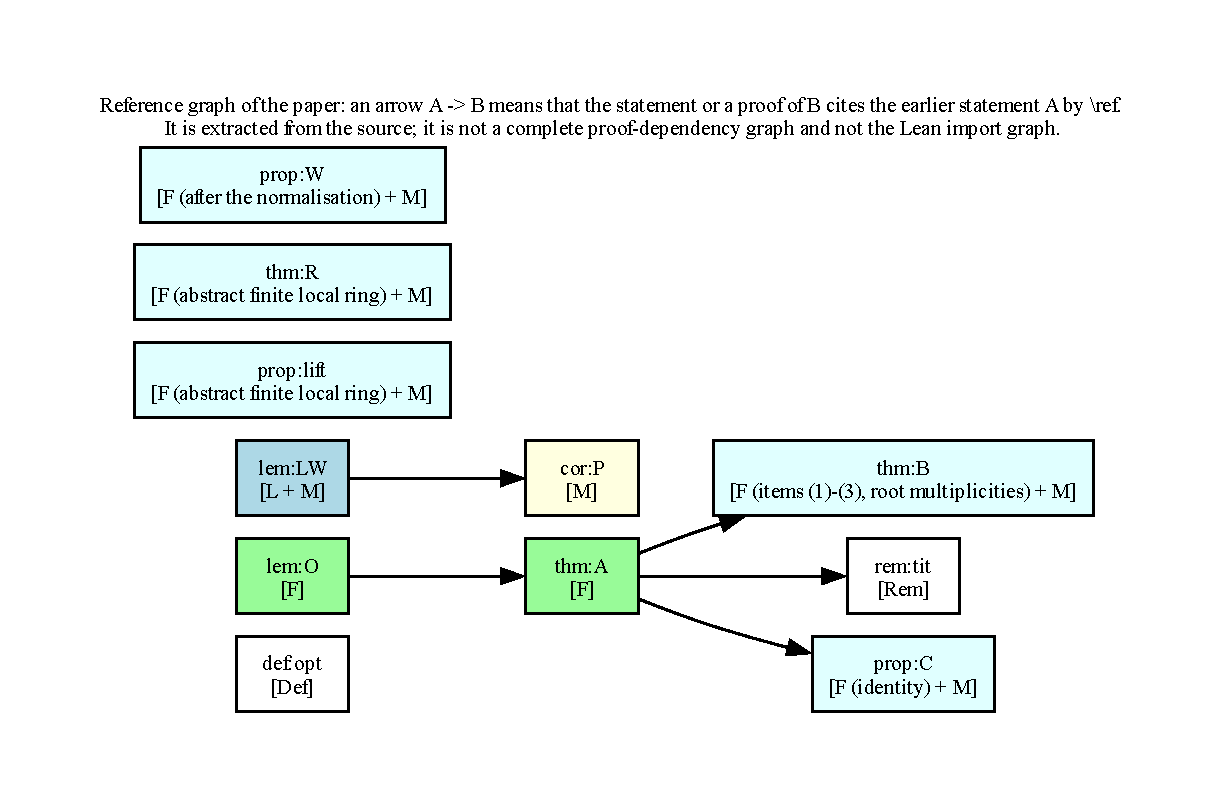
\includegraphics[width=\textwidth,height=0.42\textheight,keepaspectratio]{dep_graph.pdf}}{(Graphviz output \texttt{dep\_graph.pdf} missing.)}
\caption{Reference graph of the paper (extracted from \texttt{\string\ref} commands to earlier labelled statements). Not a complete proof-dependency graph; not the Lean import graph.}
\end{figure}
\begin{figure}[h]\centering
\IfFileExists{lean_imports.pdf}{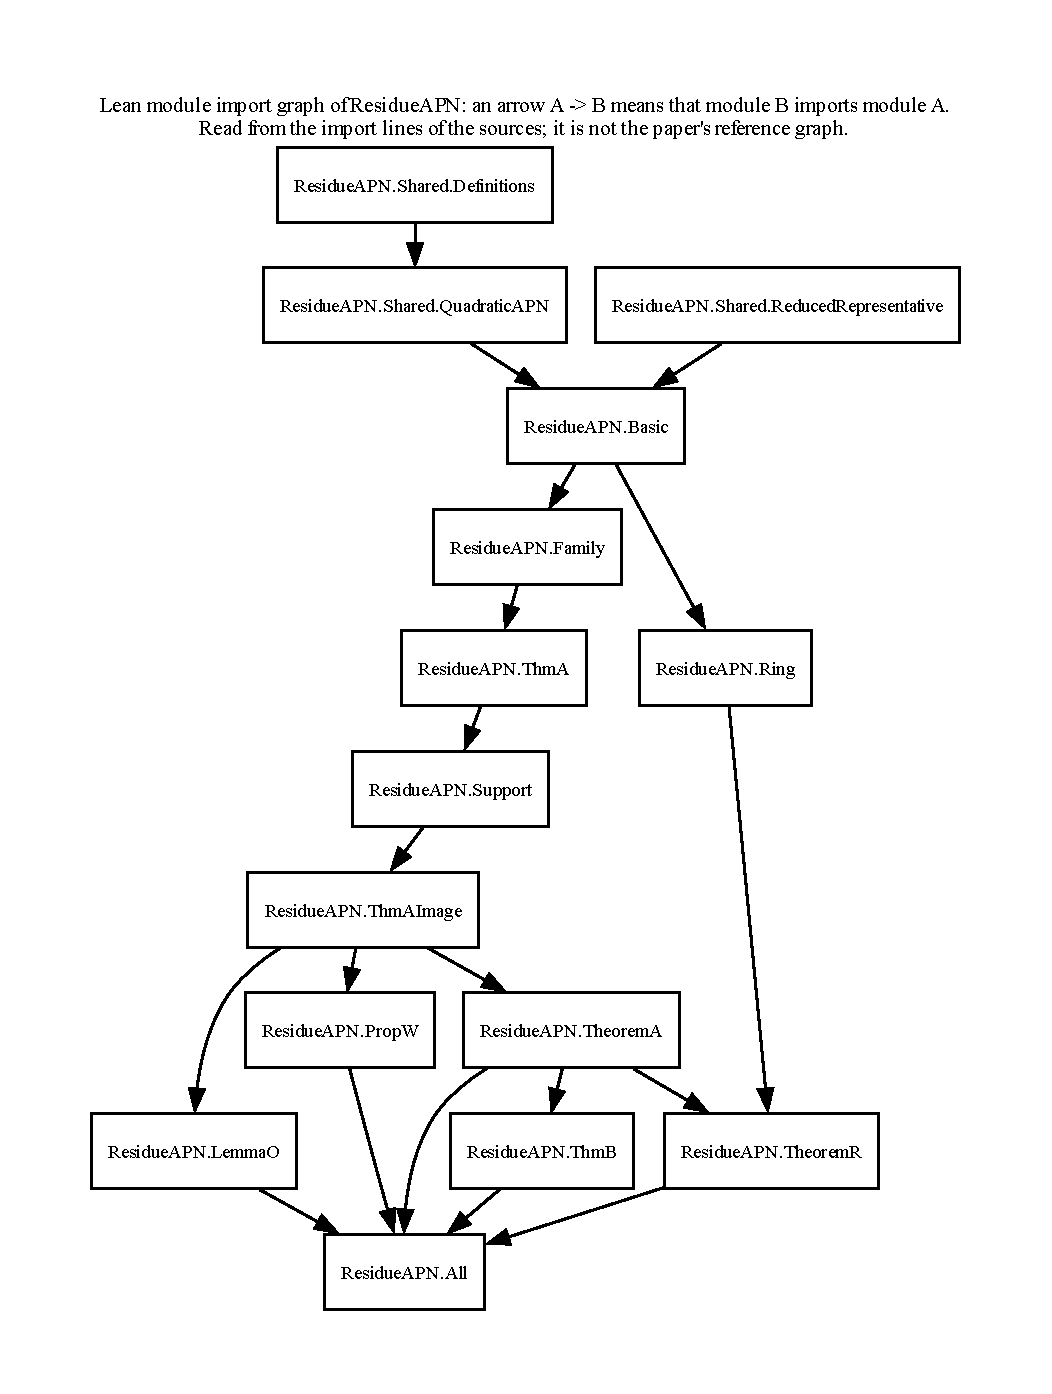
\includegraphics[width=\textwidth,height=0.42\textheight,keepaspectratio]{lean_imports.pdf}}{(Graphviz output \texttt{lean\_imports.pdf} missing.)}
\caption{Lean module import graph of \texttt{ResidueAPN} (from the import lines of the sources). Not the paper's reference graph.}
\end{figure}
% bib.tex -- GENERATED by gen_blueprint.py: the paper's bibliography, copied verbatim.
\begin{thebibliography}{9}
\bibitem{BS} D.~Bartoli and P.~St\u{a}nic\u{a}, Reduced polynomial lifts of APN permutations over Galois rings and effective non-APN bounds, preprint, arXiv:2608.30808v1, 31 August 2026, doi:10.48550/arXiv.2608.30808.
\bibitem{BL} C.~Beierle and G.~Leander, New instances of quadratic APN functions, \emph{IEEE Trans.\ Inf.\ Theory} 68(1) (2022) 670--678, doi:10.1109/TIT.2021.3120698; arXiv:2009.07204v4.
\bibitem{Chen} R.~Chen, A general approach to permutation polynomials from quadratic forms, preprint, arXiv:2506.24012v1, 2025, doi:10.48550/arXiv.2506.24012.
\bibitem{TIT} H.~Fukui, Optimal reduced representatives of quadratic APN permutations in odd dimension, submitted to \emph{IEEE Trans.\ Inf.\ Theory} (IT-26-1499); preprint, Zenodo, doi:10.5281/zenodo.23074611.
\bibitem{KZ} C.~Kaspers and Y.~Zhou, A lower bound on the number of inequivalent APN functions, \emph{J.\ Combin.\ Theory Ser.~A} 186 (2022) 105554, doi:10.1016/j.jcta.2021.105554; cited by the numbering of arXiv:2002.00673v2.
\bibitem{LW} Y.~Li and M.~Wang, On EA-equivalence of certain permutations to power mappings, \emph{Des.\ Codes Cryptogr.} 58(3) (2011) 259--269, doi:10.1007/s10623-010-9406-8.
\bibitem{RS} S.~R{\o}njom and A.~Sandrib, On the differential uniformity of polynomials over Galois rings, \emph{Cryptogr.\ Commun.} 18(6) (2026) 2057--2077, doi:10.1007/s12095-026-00895-x.
\bibitem{Stone} D.~Stone, \texttt{apn-critical-point-counterexample}, GitHub repository, created 27 September 2026, \url{https://github.com/drewstone/apn-critical-point-counterexample} (accessed 7 October 2026).
\bibitem{YKBL} Y.~Yu, N.~Kaleyski, L.~Budaghyan and Y.~Li, Classification of quadratic APN functions with coefficients in $\F_2$ for dimensions up to 9, \emph{Finite Fields Appl.} 68 (2020) 101733, doi:10.1016/j.ffa.2020.101733.
\end{thebibliography}

\end{document}
